\chapter{Fundamentos teóricos}

\section{Antecedentes}

La clasificación por medio de redes neuronales ha sido un hito ya marcado en el campo agronómico, muchos estudios se han realizado con el objetivo de analizar ciertos comportamientos de plantas y los beneficios que se puedan sacar de ellas. En 2011, el grupo de investigación de sistemas de procesamiento y control de señales de la Universidad Nacional Tenaga de Malasia desarrollo un sistema de inteligencia con un enfoque novedoso para la clasificación de frutas usando técnicas de procesamiento de imágenes digitales y redes neuronales artificiales, con el objetivo de desarrollar un método de clasificación rápido con una meta del 100\% de eficiencia. El estudio se realizó con cinco frutas, manzanas, plátanos, zanahorias, mangos y naranjas, extrayendo de ellas siete características en función de la forma y el color. La captura de las imágenes se realizó con una cámara digital convencional y las manipulaciones a los datos y construcción de la red con el software MATLAB. Los resultados obtenidos durante esta investigación fueron de gran avance en el campo de reconocimiento de patrones en imágenes.\\

En 2011, Mayabiro E presento en la Universidad Nacional Experimental del Táchira, un prototipo sobre el entorno MATLAB para el cálculo de la tasa de germinación de plántulas de pimentón previamente segmentadas. El entorno desarrollado permitía establecer una clasificación de las plántulas, hojas u objetos de la misma por medio de redes neuronales. Se realizó el entrenamiento de múltiples redes neuronales multicapas con algoritmos de retro propagación, donde aunque variaban las capas intermedias de las redes y sus funciones de transferencia fueron entrenadas con los mismos  datos de entrada, validándolas con una base de datos de pruebas para seleccionar al final una con salidas similares a las deseadas.\\

Otro estudio realizado en 2013 por Stephen Gang Wu consistía en el estudio teórico de técnicas de procesamiento de imágenes y datos para el reconocimiento automático de hojas para la clasificación de plantas. Doce características de las plantas fueron extraídos y distribuidas en cinco variables principales que constituían el vector de entrada de una red neuronal artificial pirobalística, que había sido entrenada con 1800 hojas para clasificar 32 tipos de plantas con una precisión superior al 90\%, el autor aseguraba que su metodología de implementación de la PNN era fácil y rápida en comparación de otras investigaciones similares.\\

En 2017, Bernal N realizo un estudio de campo con el cultivo de papa criolla para evaluar la influencia de la densidad de siembra asociada a distancias entre plantas de 30,40 y 50 cm y distancias entre surcos de 100 cm sobre el conteo de tubérculos de calibres inferiores a 2 cm, entre 2 y 4 cm, entre 4 y 6 cm, y de más de 6 cm de diámetro ponderado y sobre el peso fresco en gramos de los tubérculos. Los tubérculos cosechados se clasificaron y contaron mediante tamizado y se pesaron en su totalidad sin discriminar por calibre. Los modelos estadísticos empleados para modelar el comportamiento de la cosecha, evidenciaron el efecto significativo de la densidad de siembra sobre el conteo de tubérculos y calibre y se observó una razón aproximada de 40:40:20:1 desde el calibre menor al mayor. El efecto de la competición, en todos los modelos probados resulto significativo, aumentando en la mayoría de los casos a medida que disminuía la distancia entre plantas, tanto en el patrón de vecindad intrahileras como en el caso de inter e intrahileras.

\section{Bases Teóricas}

\subsection{Papa criolla (\textit{Solanum Phureja}).}

Las variables que influyen en el rendimiento de la papa pueden ser observados en la figura \ref{fig:arch}. Pag.\pageref{fig:arch}.\\
\begin{figure}[h]
	\caption{Variables de influencia sobre el rendimiento de Solanum Phureja.}
	\centering
	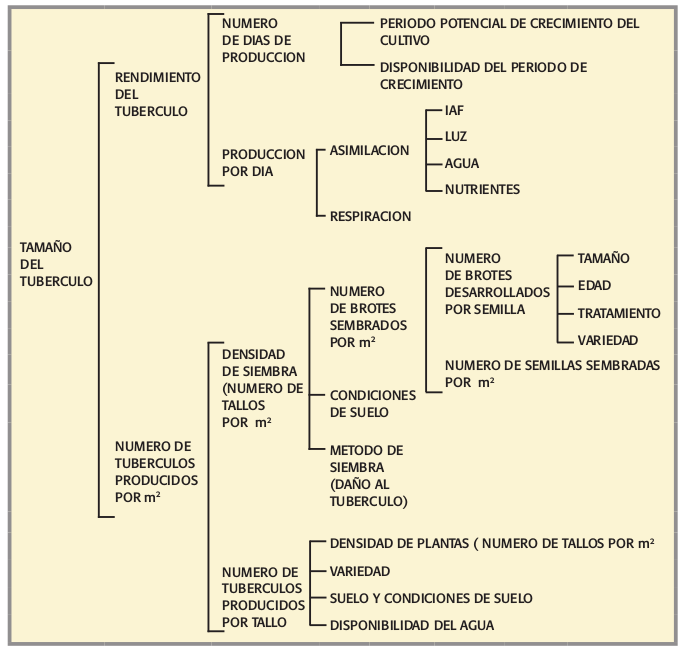
\includegraphics[scale=0.5]{variables.png}
	\label{fig:arch}
\end{figure}

\subsection{Regresión Espacial.}

El análisis exploratorio de datos espaciales - AEDE, constituye una disciplina reciente que ha adquirido una especial importancia debido principalmente al avance de la tecnología en las comunicaciones y la globalización de la economía. Los sucesos que ocurren en una ubicación específica tienen repercusiones sobre sus vecinos directos e incluso sobre otros, aparentemente remotos. \\

En el estudio de cualquier fenómeno de carácter social o económico la ubicación geográfica de los agentes constituye un aspecto importante dentro de la especificación de los modelos econométricos, ya que puede existir algún efecto espacial, que de no ser incorporado en la especificación, podría afectar la validez del modelo. Ante esta realidad y gracias al desarrollo tecnológico de los sistemas de georreferenciación de datos, surge la necesidad de contar con herramientas apropiadas para el procesamiento, descripción y análisis de la información ya que los métodos tradicionales de la estadística descriptiva no tienen en cuenta la localización geográfica de los datos.\\

Teniendo en cuenta que la econometría tradicional no ha incorporado el efecto de dichas circunstancias y que la estadística espacial se ocupa de otro tipo de problemas, ha surgido una disciplina a la cual se le ha dado el nombre de econometría espacial. Según Luc Anselin, uno de sus principales investigadores, “las actividades como la estimación de modelos espaciales de interacción, el análisis estadístico de la función de densidad urbana y la implementación empírica de modelos econométricos regionales, podrían ser considerados econometría espacial” (Anselin, 1988).\\

Cuando se tienen observaciones georreferenciadas, se deben utilizar herramientas que permitan detectar ciertas características dentro de los datos, como son tendencia, valores atípicos, esquemas de asociación y
dependencia espacial, concentración espacial o puntos calientes/fríos, entre otros.\\
Aunque en la actualidad se tiene gran cantidad de información georreferenciada, estos datos suelen ser tratados con herramientas del análisis de series temporales (o de corte transversal, no espacial), sin usar técnicas adecuadas para el análisis estadístico espacial. Los métodos que permiten extraer dichas características de los datos georreferenciados se conocen con el nombre de análisis exploratorio de datos espaciales (AEDE) y se conciben como una disciplina dentro del análisis estadístico más general, diseñada para el tratamiento específico de los datos geográficos. El AEDE se utiliza para identificar relaciones sistemáticas entre variables, o dentro de una misma variable, cuando no existe un conocimiento claro sobre su distribución en el espacio geográfico (Chasco Yrigoyen, 2006).

\subsection{Redes Neuronales Artificiales.}

Una red neuronal artificial (ANN) es un conjunto de nodos de un programa (neuronas) interconectados entre sí, simulando el proceso de pensamiento humano, se pudiera considerar como una caja negra entrenada previamente para esperar una entrada y basado en las características o comportamiento de la misma proporcionar una determinada salida, eliminando así la necesidad de diferentes algoritmos que deban analizar comportamientos cada uno por separado. Una red neuronal probabilística (PNN) no es más que una ANN que usa funciones estadísticas que escalan la variable no linealmente como una forma de campana o una distribución normal (Stephen, 2007).\\

Entre las definiciones más recientes de inteligencia artificial se expresa, en forma general, la inteligencia artificial como la capacidad que tienen las máquinas para realizar tareas que en el momento son realizadas por seres humanos; otros autores como Nebendah (1988) y Delgado (1998) dan definiciones más completas y las definen como el campo de estudio que se enfoca en la explicación y emulación de la conducta inteligente en función de procesos computacionales basados en la experiencia y el conocimiento continuo del ambiente. Autores como Marr (1977), Mompin (1987), Rolston (1992), en sus definiciones involucran los términos de soluciones a problemas muy complejos.\\

El nacimiento de la inteligencia artificial se sitúa en los años cincuenta; en esa fecha la informática apenas se había desarrollado, y ya se planteaba la posibilidad de diseñar máquinas inteligentes. Hoy en día se habla de vida artificial, algoritmos genéticos, computación molecular o redes neuronales. En algunas de estas ramas los resultados teóricos van muy por encima de las realizaciones prácticas.\\

A través de los años, se han utilizado diversas técnicas de inteligencia artificial para emular 'comportamientos inteligentes'. Al software que hace uso de dichas técnicas se le denomina, de forma genérica, 'sistema inteligente', y es cada vez más amplía la gama de aplicaciones financieras donde incide la inteligencia artificial.\\

Un ejemplo de esto es que al usarse una tarjeta de crédito, suelen acumularse datos sobre patrones de consumo que después se venderán a diversas empresas. Sobre la base de los pagos efectuados en dicha tarjeta de crédito, los bancos e instituciones de crédito irán elaborando un historial del usuario, el cual se utilizará para autorizar una transacción, para decidir cuándo extender el crédito y para detectar fraudes. Este tipo de procesos requiere de chequeos que suelen resultar bastante complejos, además del uso de criterios variables para poder tomar una decisión final en torno a la autorización de una cierta transacción. Claro que, al manejar enormes volúmenes de información, como los aproximadamente 16 millones de transacciones que Visa Internacional debe verificar diariamente, no resulta nada fácil poder detectar un fraude. Aunque es evidente la necesidad de automatizar procesos como éste, no es del todo obvio incorporar el comportamiento inteligente del ser humano a un programa de computadora que reemplace a un evaluador humano, ya que los sistemas de inteligencia artificial se toman como herramientas de apoyo analítico para el evaluador, mas no como una unidad autosuficiente que por sí sola pueda tomar decisiones.\\

Las redes neuronales artificiales son eficientes en tareas tales como el reconocimiento de patrones, problemas de optimización o clasificación, y se pueden integrar en un sistema de ayuda a la toma de decisiones, pero no son una panacea capaz de resolver todos los problemas: todo lo contrario, son modelos muy especializados que pueden aplicarse en dominios muy concretos.\\

Las redes neuronales emulan la estructura y el comportamiento del cerebro, utilizando los procesos de aprendizaje para buscar una solución a diferentes problemas; son un conjunto de algoritmos matemáticos que encuentran las relaciones no lineales entre conjuntos de datos; suelen ser utilizadas como herramientas para la predicción de tendencias y como clasificadoras de conjuntos de datos. Se denominan neuronales porque están basadas en el funcionamiento de una neurona biológica cuando procesa información.

\subsection{Curvas ROC.}

Una amplia gama de test diagnósticos reportan sus resultados cuantitativamente, utilizando escalas continúas. El análisis de curvas ROC (receiver operating characteristic curve) constituye un método estadístico para determinar la exactitud diagnóstica de estos test, siendo utilizadas con tres propósitos específicos: determinar el punto de corte de una escala continua en el que se alcanza la sensibilidad y especificidad más alta, evaluar la capacidad discriminativa del test diagnóstico y comparar la capacidad discriminativa de dos o más test diagnósticos que expresan sus resultados como escalas continuas.

\subsection{Lenguaje R.}

R es un conjunto  integrado de \textit{software} de código abierto para el almacenamiento, manipulación, cálculo y visualización de datos para computación y graficación estadística, puede ser compilado y ejecutado en Windows, Mac OS X y otras  plataformas UNIX (como Linux), se distribuye usualmente en formato binario (\url{https://www.r-project.org/about.html}, 2018). El proyecto de \emph{software} R fue iniciado por Robert Gentleman y Ross Ihaka. El lenguaje fue influenciado por  lenguaje S desarrollado originalmente en Bell Laboratories por John Chambers y sus colegas. Desde entonces ha evolucionado  para el cálculo estadístico asociado a diversas disciplinas para contextos académicos y comerciales. En R, la unidad fundamental de código compartible es el paquete, el cual agrupa código, datos, documentación y pruebas, y resulta simple de compartir con otros. Para enero del 2015 ya habían más de 6.000 paquetes disponibles en la Red Integral de Archivos de R, conocido comúnmente por su acrónimo CRAN, el cual es el repositorio de paquetes . Esta gran variedad de paquetes es una de las razones por las cuales R es tan exitoso, pues es probable que algún investigador o académico ya haya resuelto un problema en su propio campo usando esta herramienta, por lo que otros usuarios simplemente podrán recurrir a ella para su uso directo o para llamarla en un nuevo código (Wickham,2015). \\

\subsection{Estructura de paquetes en R/RStudio.}

Requerimiento del núcleo (\textit{core})

\begin{enumerate}
  \item  DESCRIPTION: metadatos del package .\\
La tarea del archivo Description es de gran importancia ya que es en el donde se registra la metadata, las dependencias que utiliza el paquete, la licencia y el soporte en caso de ocurrir errores con el mismo
La estructura mínima para realizar un paquete en R es la siguiente:

\begin{itemize}
\item Package: mypackage
\item Title: What The Package Does (one line, title case required)
\item Version: 0.1
\item Authors@R: person("First", "Last", email = "first.last@example.com",
\item role = c("aut", "cre"))
\item Description: What the package does (one paragraph)
\item Depends: R (>= 3.1.0)
\item License: What license is it under?
\item LazyData: true
\end{itemize}
  \item \url{R /:} dirección del repositorio donde se encuentra el código del paquete (.R files).\\
Se expondrán las buenas prácticas a la hora de realizar todo nuestro código en R, desde organización de las funciones, estilos de código y nombre de variables 

\textbf{Organizar funciones en R:} aunque puedes organizar los archivos como desees, los dos extremos son malos no colocar todas las funciones en el mismo archivo y no crear un archivo para para función, aunque si una función es muy grande o tiene mucha documentación se puede dar el caso, los nombres de los archivos tienen que ser significado y deben de terminar en R.
\begin{itemize}
\item Bien  
\begin{itemize}
     \item fit\_models.R
     \item utility\_functions.R
  \end{itemize}
\item Mal
   \begin{itemize}
      \item foo.r
      \item stuff.r
    \end{itemize}
 \end{itemize}
Se puede recomendar de acuerdo al número de función utilizar prefijo 

\textbf{Nombres de Objetos:} Los nombres de las Variables y funciones deben de ser en minusculas, usar el guion bajo ( \_ ) para separar palabras  
\begin{itemize}
\item Bien  
\begin{itemize}
     \item day\_one
     \item day\_1
  \end{itemize}
\item Mal
   \begin{itemize}
      \item first\_day\_of\_the\_month
      \item DayOne
      \item dayone
      \item djm1
    \end{itemize}
 \end{itemize}
En lo posible no usar nombres de variables existentes esto causara confusión.

\textbf{Espaciado:} Se recomienda colocar espacios alrededor de todos los operadores lógicos y aritméticos (=, +, -, \textless-, etc.). siempre coloque un espacio después de una coma, y nunca antes de ella.

\begin{itemize}
\item Bien  
\begin{itemize}
     \item average \textless- mean(feet / 12 + inches, na.rm = TRUE)
  \end{itemize}
\item Mal
   \begin{itemize}
      \item average\textless-mean(feet/12+inches,na.rm=TRUE)
   \end{itemize}
 \end{itemize}
 
Hay una pequeña excepción a esta regla: ( :, :: y :::) no necesitan espacios alrededor de ellos.

\begin{itemize}
\item Bien  
\begin{itemize}
     \item x \textless- 1:10
     \item base::get
  \end{itemize}
\item Mal
   \begin{itemize}
      \item x \textless- 1 : 10
     \item base :: get
   \end{itemize}
 \end{itemize}

Dejar un espacio antes del paréntesis izquierdo, excepto en la llamada a una función

\begin{itemize}
\item Bien  
\begin{itemize}
     \item if (debug) do(x)
     \item plot(x,y)
  \end{itemize}
\item Mal
   \begin{itemize}
      \item if(debug)do(x)
     \item plot(x, y)
   \end{itemize}
 \end{itemize}

Se utiliza más de un espacio es caso que de mejore a la alineación, por ejemplo:\\
\begin{list}{}{}
\item list(
    \begin{list}{}{} 
       \item total \hspace{3mm}= a + b + c,
       \item mean \hspace{2mm}= (a + b + c) / n
    \end{list}
\item )
\end{list}
No coloque espacios alrededor del código entre paréntesis o corchetes (a menos que haya una coma)
\begin{itemize}
\item Bien  
\begin{itemize}
     \item if (debug)  do(x)
     \item diamonds[5, ]
  \end{itemize}
\item Mal
   \begin{itemize}
      \item if ( debug ) do(x) \textit{\# no espacios alrededor de debug}
      \item x[1,] \textit{\# necesita un espacio después de la coma}
      \item x[1 ,] \textit{\# el espacio va después de la coma no antes}	   
\end{itemize}
 \end{itemize}

\textbf{Llaves:} Una llave de apertura nunca debe ir en su propia línea y siempre debe ir seguida de un nueva línea. Una llave siempre debe ir en su propia línea, a menos que sea seguido por otra y siempre sangría el código dentro de las llaves
\begin{itemize}
\item Bien  
\begin{itemize}
     \item \begin{list}{}{} 
		\item if (y \textless  \hspace{1mm} 0 \&\&  debug) \{
		\begin{list}{}{}
		\item message(``Y es negativo")
		\end{list}
		\item \}	
	    \end{list}

       \item \begin{list}{}{} 
		\item if (y ==  \hspace{1mm} 0 ) \{
		\begin{list}{}{}
		   \item log(x)
		\end{list}
		\item \} else \{
		\begin{list}{}{}
		  \item y \^~  x
		\end{list}
		\item \}	
	    \end{list}
  \end{itemize}
\item Mal
   \begin{itemize}
     \item \begin{list}{}{} 
		\item if (y \textless  \hspace{1mm} 0 \&\&  debug)
		\item message(``Y es negativo")
	    \end{list}

       \item \begin{list}{}{} 
		\item if (y ==  \hspace{1mm} 0) \{
		\begin{list}{}{}
		   \item log(x)
		\end{list}
		\item \}
		\item else \{
		\begin{list}{}{}
		  \item y \^~  x
		\end{list}
		\item \}	
	    \end{list}   
\end{itemize}
 \end{itemize}

Sentencias  muy cortas está bien dejarla en la misma linea.\\
if(y \textless \hspace{1mm} 0 \&\& debug) message(``Y es negativo")\\

\textbf{Longitud de Linea:} cada línea debe de llevar máximo 80 caracteres, si se queda sin espacio es recomendable utilizar una función separada\\

\textbf{Sangria:} Utilice sangría de 2 espacios, nunca use tabulador o múltiples tabuladores o espacios la única excepción es cuando se define una sentencia en múltiples líneas.\\
\begin{tabular}{ccc}
long\_function\_name \textless- function(& a = ``a long argument", \\ 
 &  b = ``another argument", \\
 &  b = ``another argument", \\
\end{tabular}
\newline

\textbf{Asignacion:} Usar el \textless-, y no =
\begin{itemize}
\item Bien  
\begin{itemize}
     \item x \textless- 5
  \end{itemize}
\item Mal
   \begin{itemize}
      \item x = 5
   \end{itemize}
 \end{itemize}

  \item man/: documentación.\\
  \item NAMESPACE: específica que objetos conforman el paquete.\\
\end{enumerate}
\textbf{Comentarios:} Comente tu código, el comentario comienza \#, los comentarios deben de explicar el porqué, no el que.\\ use los caracteres (-) y (=) para separar líneas\\
{\# Load data - - - - - - - - - - - - - - - - - - - - - - - - - - - - - - - - - - - - - -}\\
{\# Plot data - - - - - - - - - - - - - - - - - - - - - - - - - - - - - - - - - - - - - - -}\\


\subsection{RStudio.}

RStudio es un ambiente de desarrollo integrado (\textit{Integrated Development Environment}, IDE) que ofrece herramientas de desarrollo vía consola, editor de sintaxis que apoya la ejecución de código, así como herramientas para el trazado, la depuración y la gestión del espacio de trabajo.  RStudio está disponible para Windows, Mac y Linux o para navegadores conectados a RStudio Server o RStudio Server Pro (Debian / Ubuntu, RedHat / CentOS, y SUSE Linux) (\url{https://www.rstudio.com/about/}, 2018).
 

